\section{Neural Networks}
Neural Networks are functions \(y = f(x,\theta)\) with parameters \(\theta\) that map mulitvariate inputs \(x\) to mulitvariate outputs \(y\).

\textbf{Unversal approximation theorem:} A shallow neural network (MLP) using nonlinear activation function can approximate any given continuous function defined ib a compact subset of \(R^D\) to arbitrary precision given enough hidden units (finite number).

\subsection{Loss function}
Regression: Mean squared error loss
\[
MSE = \frac{1}{N}\sum_{i=1}^{N}(y_i- \hat{y}_i)^2
\]
Classification: Cross entropy loss
\[
Loss = -\sum_{i= 1}^{\text{\#output classes}}y_i \cdot \log(\hat{y}_i)
\]
\subsection{Training}
Repeat:
\begin{itemize}
    \item Choose a training sample
    \item Forward pass: Compute the prediction
    \item Backward pass: If error > 0, update weights
\end{itemize}
Adjust weigths by Gradient descent
\[
w_i = w_i - \alpha\frac{\partial J(w_i)}{\partial w_i}
\]

Training Terms:
\begin{itemize}
    \item Epoch = a forward pass and backward pass complete for all the training examples
    \item Batch size = the number of training samples in a Batch
    \item Iteration = forward and backward pass each using a Batch
    \item Iterations per Epoch = \#training data /size of Batch
\end{itemize}
 Avoide overfitting with:
 \begin{itemize}
    \item Regularization (Lasso, Ridge)
    \item Dropout, turn off some neurons during training
    \item Batch normalization
    \item Early stopping
 \end{itemize}

 \subsection{Convolutional Neural Networks (CNN)}
 Idea: nearby pixels in an image are correlated - using shared parameters across whole input.
 A convolution operation is determined:
 \begin{itemize}
     \item stride (kernel shift)
     \item kernel size (typically odd)
     \item dilation (number of zero weights in kernel)
 \end{itemize}
 Convolutional Layer: apply convolution, add bias, apply activation function.

 Channels(feature maps, activation maps): mulitple convolutions applied to the input in parallel.
\subsubsection{CNN 1D}
\begin{figure}[!h]
    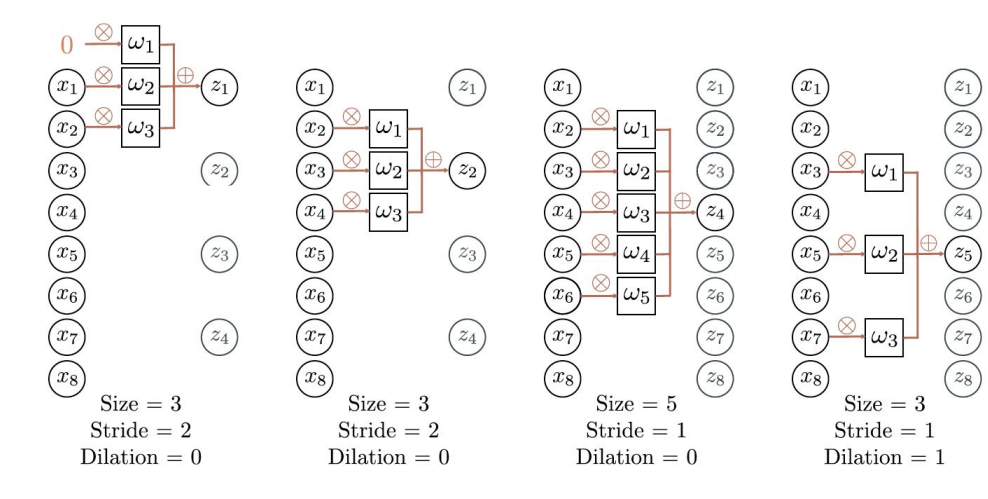
\includegraphics[width = \columnwidth]{figures/06/1DConv.png}
 \end{figure}
1D convolution is a weighted sum of nearby inputs.

\subsubsection{CNN 2D}
Using 2D kernles, plus a bias and a activation function.
\begin{figure}[!h]
    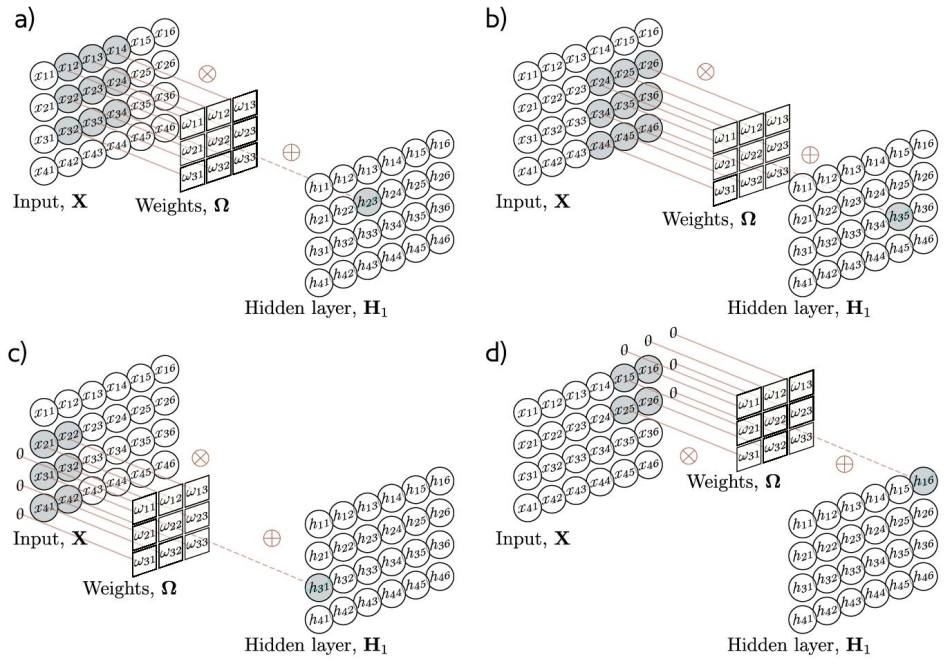
\includegraphics[width = \columnwidth]{figures/06/2DConv.png}
 \end{figure}

 \subsubsection{Pooling}
 Reduces Dimensions by min,max or average pooling a layer.
 \begin{figure}[!h]
    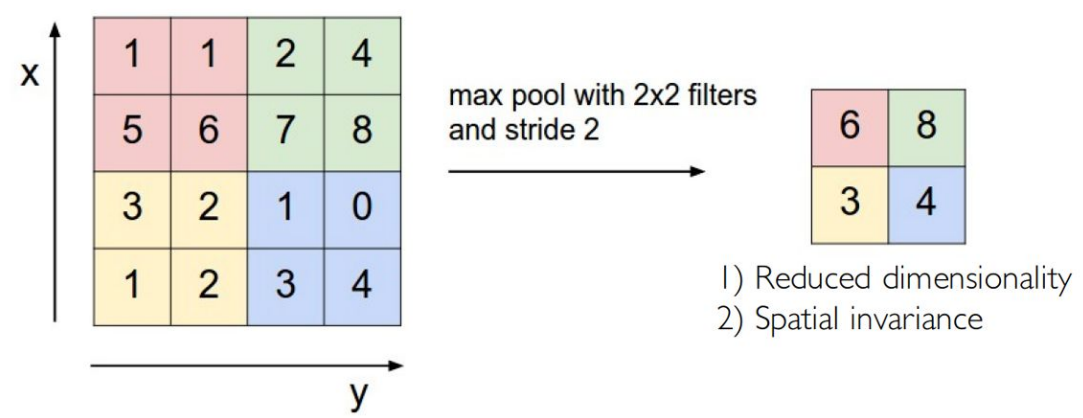
\includegraphics[width = \columnwidth]{figures/06/Pooling.png}
 \end{figure}
 \subsubsection{Transpose Convolution}
 Upsampling: Each input contributed multiple times to the output.
 Useful when output is an image.